\subsection{The need for smoothing}
\label{sec:need for smoothing}
Let $\formula$ be an MTL formula with horizon $N$.
We aim to solve the problem
\begin{eqnarray}
\label{eq:min rob problem}
\max_{x_0 \in X_0, \inpSig \in \inpSet^{N-1}, \sstraj \in X^N} && \robf(\sstraj)
\nonumber
\\
\text{s.t. } && x_{t+1} = f(x_t,u_t) \; \forall t=0,1,\ldots,N-1
\end{eqnarray}
using established, powerful gradient descent algorithms \cite{Polak97_Optim}, rather than heuristics like Simulated Annealing \cite{kirkpatrickV_SA83}.
Gradient descent algorithms typically offer convergence guarantees to the function's minima, have known convergence rates for certain function classes, and have been optimized so they outperform heuristics that don't have access to the objective's gradient information.
Moreover, they usually have a fewer number of parameters to be set by the user, and important issues like step-size selection are rigorously addressed.

To apply gradient descent methods, we require a differentiable objective function. 
Our objective function, $\robf$, is non-differentiable, because it uses the distance function, and max and min functions, all of which are non-differentiable.
One may note that these functions are all differentiable almost everywhere (a.e.).
That is, the set of points in their domain where they are non-differentiable has measure 0 in $\Re^n$. 
Therefore, by measure additivity, the composite function $\robf$ is itself differentiable almost everywhere.
Thus, one may be tempted to `ignore' the singularities (points of non-differentiability), and apply gradient descent to $\robf$ anyway.
The rationale for doing so is that sets of measure 0 are unlikely to be visited by gradient descent, and thus don't matter. 
However, as we show in the next example, the lines of singularity (along which the objective is non-differentiable) can be  precisely the lines along which the objective increases the fastest.
See also \cite{Cortes08_Discontinuous}.
Thus they are consistently visited by gradient descent, after which it fails to converge because of the lack of a gradient.


\begin{exmp}
	\label{ex:cluster nondiff}
	We use Sequential Quadratic Programming (SQP) \cite{Polak97_Optim} to maximize robustness of a single point, $x\in \mathbb{R}^2$, with respect to an unsafe set, $[-1,1]^2$ (in red in Fig. \ref{fig:DumbExample}), with $x$ constrained to a set $[-2.5,2.5]^2$ (in grey in Fig. \ref{fig:DumbExample}). We initialize the SQP from the point $x_0=[0\,0]'$, which corresponds to a robustness of $-1$, the minima in this (maximization) problem. In this problem, it is clear the optimal solution(s) lies at the boundary of the gray set, i.e. at a maximum possible distance from the unsafe set. SQP with the cost of maximizing the robustness function gets stuck at a local minima, corresponding to $x=[1\,1]'$ as shown in Fig. \ref{fig:DumbExample}. 
	
	\todo[inline]{Habbas, can you explain the reason why? Eloquently please. Also note that our method gets to a global optimal (the green point).} 
\begin{figure}[t]
\centering
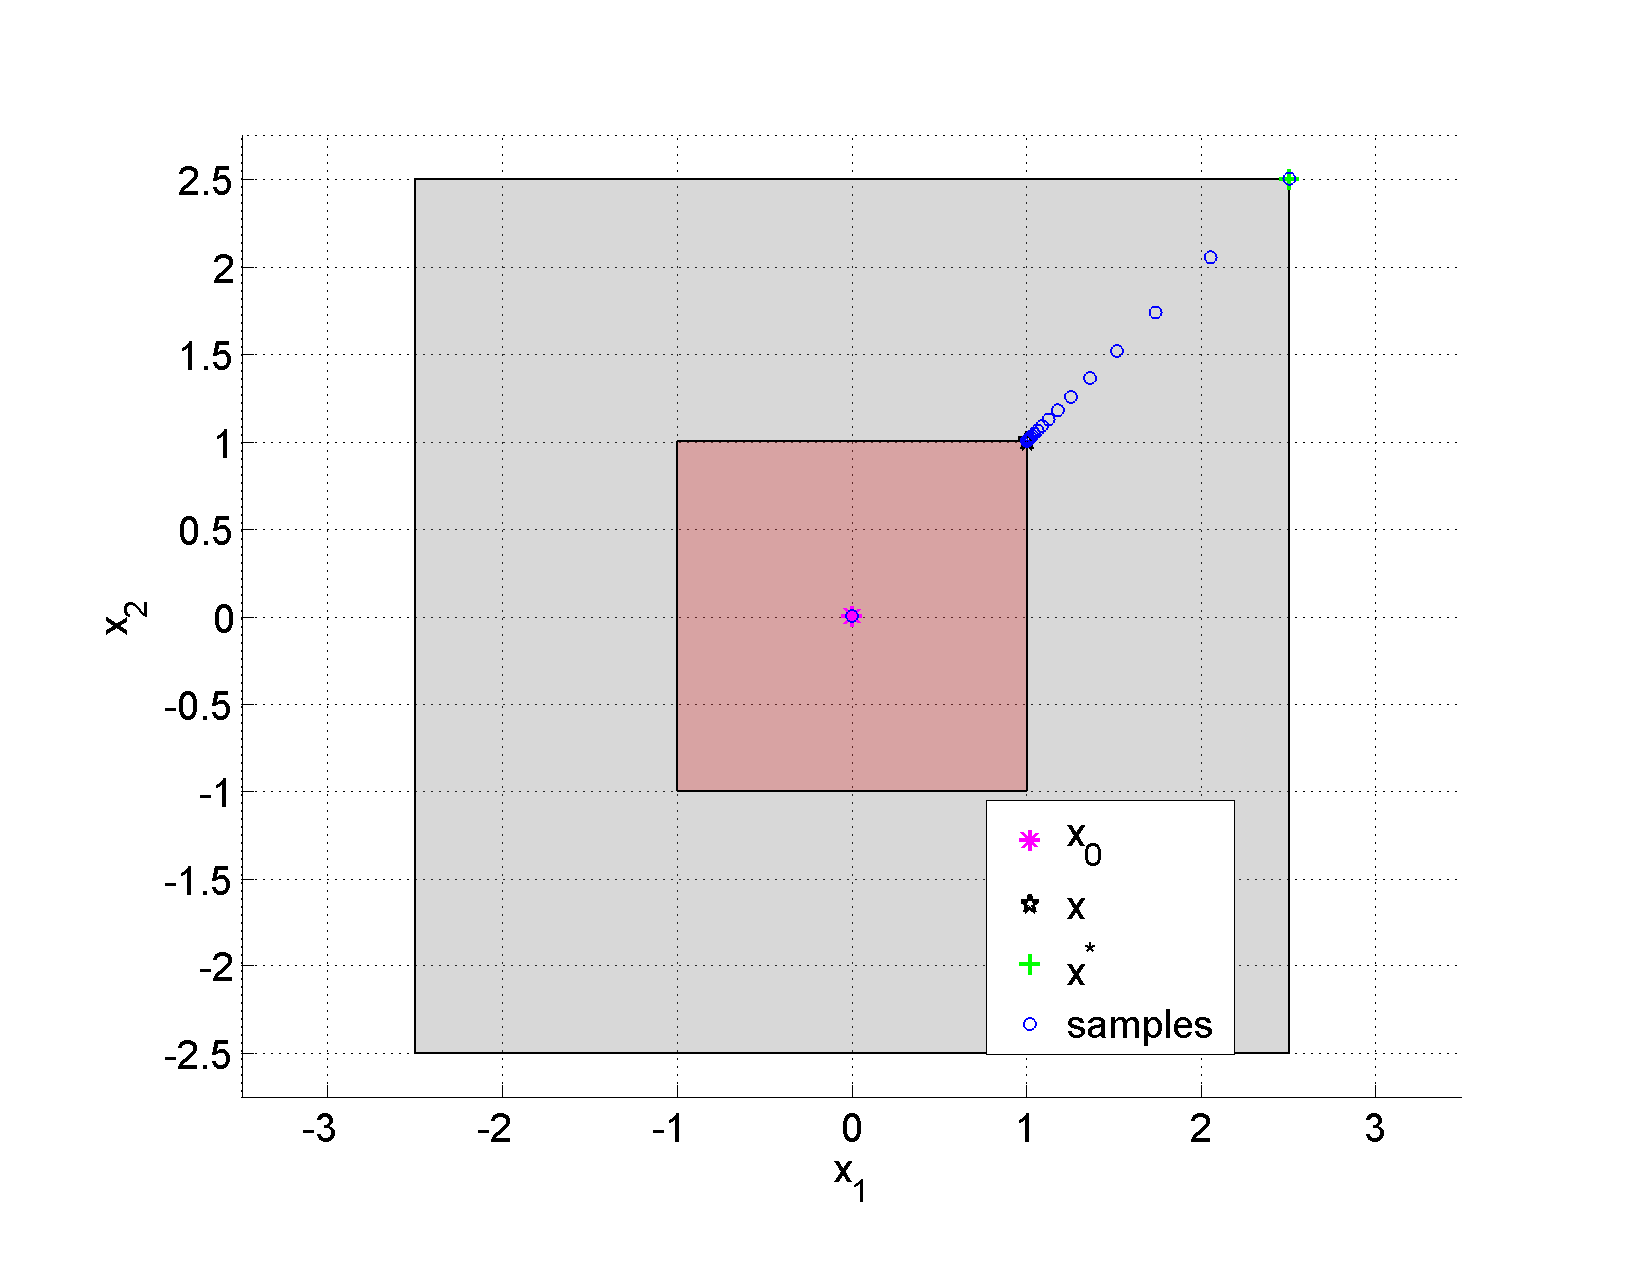
\includegraphics[width=0.49\textwidth]{figures/DumbOptEx}
\caption{Iterates of SQP for Example \ref{ex:cluster nondiff}}
\label{fig:DumbExample}
\end{figure}

\end{exmp}
